\section{Proposed technical architecture and challenges}
As an organization covering areas like research, student affairs and administration a university has to manage a significant amount of knowledge, adding new information on a daily basis.
Such an application domain is complex and includes areas like management of an academic library and provision of educational resources which have to be conform with stakeholders requirements. Traditionally the \textit{Service Oriented Architectures~(SOA)} have been used to meet these needs. However, as the application domain grows many small and similar services tend to emerge. That phenomena can not only be observed at the Vienna University of Technology, but also at the Open University\footnote{\url{http://www.open.ac.uk/}}~\cite{inproceedings:zablith_consuming_2011}.

A major problem of evolving similar, independent services are diverging data formats and service owners. Thus, knowledge and administrative information that has been collected by multiple services can not be easily interlinked. An example for such isolated services is the e-learning platform called TUWEL\footnote{\url{https://tuwel.tuwien.ac.at/}}, combining moodle\footnote{\url{https://moodle.org/}} and the central information system called TISS\footnote{\url{https://tiss.tuwien.ac.at/}}. These services provide course information and material, but are intended for different purposes. Whereas TISS focuses mainly on administrative functionality, TUWEL supports the interaction between teacher and student. 
Adding additional services which, for example, synchronize deadlines and registration dates is costly due to the fact that the information is separated over different isolated sources and not easily accessible. 

\subsection{The big picture}

\begin{figure}[htbp]
\centering
{\scalebox{0.7}{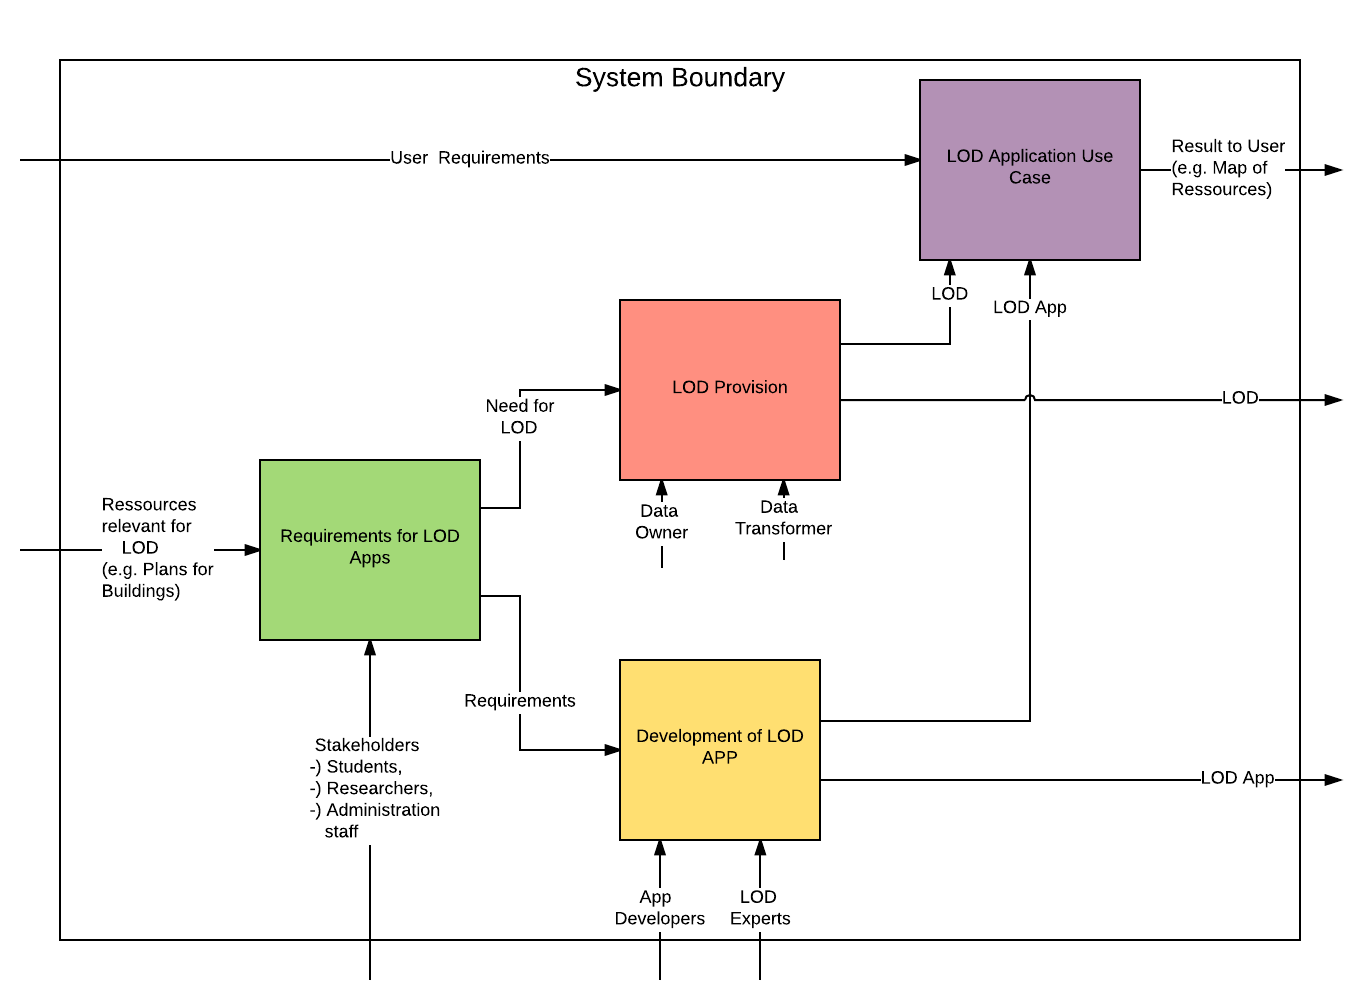
\includegraphics{images/architecture/idef0.PNG}}}
\caption[High level framework for LOD publishing]{High level framework for LOD publishing in IDEF0 notation}
\label{Fi:idef0}
\end{figure}
\subsubsection{Parts}
In this sub-section we provide an overview of a high level architecture, illustrated
in Figure~\ref{Fi:idef0}, for a university wide publication framework which includes:

\begin{itemize}
	\item \textbf{Requirements for LOD-Applications}\newline
	At the beginning stand the existing resources and the needs of the stakeholder. Combining these leads to the requirements for an application, the first step of the process. According to this requirement a decision has to be made whether they are  realizable depending on the cost-value ratio and whether the solution has to be a LOD application. These process has to actively involve all stakeholders.
	\item \textbf{Data Provision}\newline
	After defining the requirements, the existing data (e.g. a publication database) must be transformed in a appropriate, machine readable LOD format. These can happen in a manually (only for small data sets) or a (semi-)automated (for big data set) way. Ideally there is a automated transformer based on an existing, well maintained and up-to-date database so there has to be less cared about the of the data (for a more technical description see Section~\ref{subsubsec:integration}). Key roles for this process are the original data owner and the data transformer.
	\item \textbf{Development of an Application}\newline
	Based on the requirements definitions from the previous step a proper application (e.g. a browser of publication data) now can be constructed considering the stakeholder needs and existing resources (transformed to LOD).  To support this process and to not obtaining all knowledge from zero it is recommended to access the knowledge of LOD experts (e.g. provided by the LinkedUniversities~\footnote{\url{www.linkeduniversities.org/}}). The development can simultaneously be done with the data provision if proper interface between the application and its data are made. 
	\item \textbf{Application Use Case}\newline
	Combining the data, transformed in LOD, the LOD application and user requirements (not the application requirements from the first step) result in the actual application use case, representing the environment or the domain.
\end{itemize}

\subsubsection{In- and outbound interfaces}

There were several indirectly interfaces mentioned above - we define them now in a more formal way and divide them in inbound (arrows pointing from outside the system boundary) and outbound interfaces (arrows pointing from inside the system boundary).

The inbound interfaces are:

\begin{itemize}
	\item \textbf{User Requirements}\newline
	Understanding user requirements is an essential part of the software development process. Due to the open nature of Linked Open Data privacy concerns and legal issues should be already considered in the requirements as misunderstandings are hard to fix in later phases.
	\item \textbf{Existing Resources}\newline
	The starting point of every LOD application are resources, ideally already existing (to reduce the amount of work). It can be everything from relational databases, simple Excel files or other Linked (Open) Data sets. For more details see section~\ref{subsubsec:sources}.
	\item \textbf{Stakeholders}\newline
	Stakeholders are defined as \textit{"`a person, group or organization that has interest or concern in an organization. Stakeholders can affect or be affected by the organization's actions, objectives and policies."'}~\cite{book:Post2002} Their needs and demands have to be considered in a LOD project as similar as in every other software project.
	\item \textbf{Application Developers}\newline
	\item \textbf{LOD Experts}\newline
	To avoid unnecessary redundancy in acquiring knowledge of LOD implementation, it is highly recommended to involve either LOD experts in the development or access their accumulated know-how e.g. by platforms like LinkedUniversities~\footnote{\url{www.linkeduniversities.org/}} (see section~\ref{linkeduniversities})
	\item \textbf{Data Owner}\newline
	Every data set has its owner, therefore this role has to be considered in the development process to avoid organizational conflicts and copyright issues. Ideally he is directly involved to access his specific know-how about the data set.
	\item \textbf{Data Transformer}\newline
	To use a data set in a LOD approach, the data have to be transformed either manually or (semi-)automatically into a proper format (see~\cite{artivle:bernerslee-t-2006-1} for the 5 star model of data format and section~\ref{subsubsec:integration} for details about transformations).
\end{itemize}

The outbound interfaces are:

\begin{itemize}
	\item \textbf{Linked Open Data}\newline
	As a result of the LOD provision the actual data are provided e.g. as SPARQL endpoint, so others can easily access and use them in other applications. For technical details about endpoints see section~\ref{subsubsec:provision} or as example the SPARQL endpoint of The Open University~\url{www.data.open.ac.uk/query}.
	\item \textbf{Application}\newline
	The outcome of the development phase are applications for end-users to access and interact with the data e.g. in form of an web platform. For technical details about endpoints see section~\ref{subsubsec:application} or as example the application list of The Open University~\url{www.data.open.ac.uk/applications.html}.
	\item \textbf{End-User Result}\newline
	Finally the main result is the actual interaction of the users with the applications and endpoints, (hoepfully) acting in the boundaries of the defined use cases.
\end{itemize}

\subsection{Proposal of a technical architecture}

\begin{figure}[htbp]
\centering
{\scalebox{0.5}{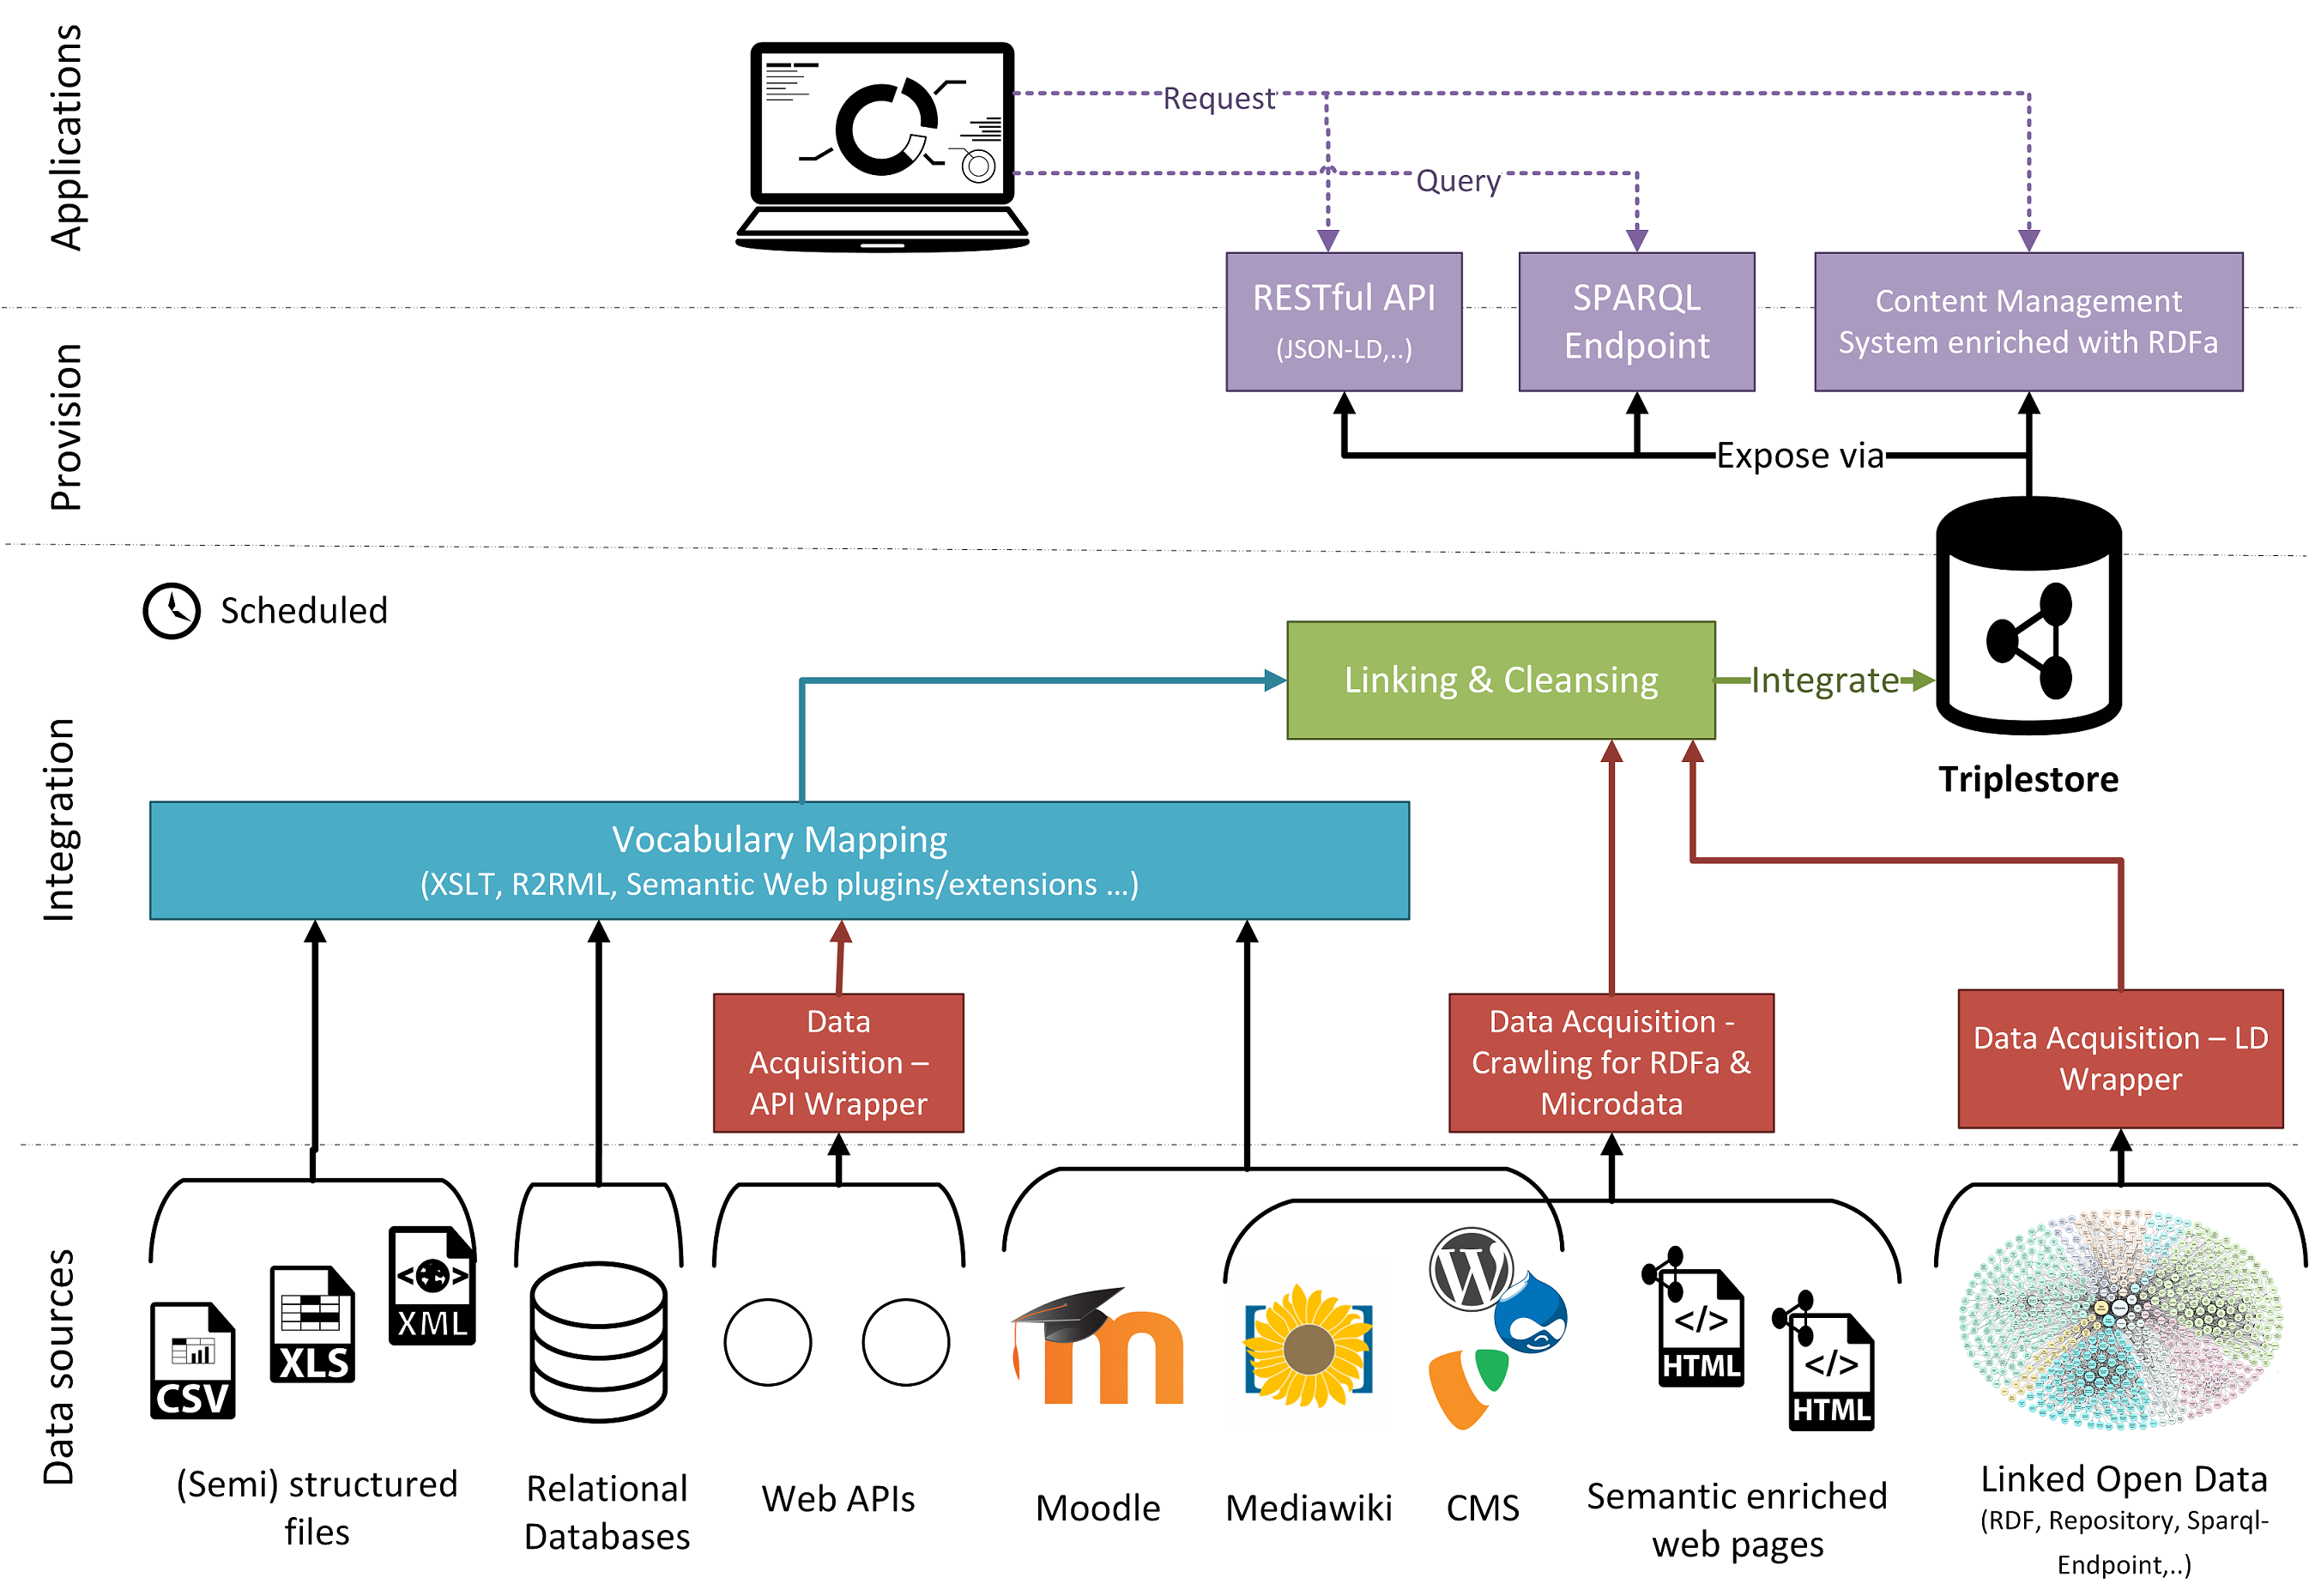
\includegraphics{images/architecture/lod_technical_architecture.PNG}}}
\caption[High level technical architecture of a LOD system]{High level technical architecture of a LOD system //TODO: source}
\label{Fi:tec_architecture}
\end{figure}

\subsubsection{Data sources}\label{subsubsec:sources}
\subsubsection{Integration}\label{subsubsec:integration}
\subsubsection{Ontologies}\label{subsubsec:ontologies}
\subsubsection{Provision}\label{subsubsec:provision}
\subsubsection{Application}\label{subsubsec:application}

\subsection{Stakeholder specific issues (datasets, application types)}
\subsection{Challenges}
\subsubsection{Data ownership}
\subsubsection{Data quality}